\documentclass[10pt,a4paper]{report}
\usepackage[utf8x]{inputenc}
\usepackage{ucs}
\usepackage{amsmath}
\usepackage{amsfonts}
\usepackage{amssymb}
\usepackage{makeidx}
\usepackage{graphicx}
\usepackage[brazil]{babel}
\usepackage{hyperref}
\usepackage{pdfpages}
\author{Vagner Clementino}
\title{Relatório de Progresso do Mestrado\\
	Vagner Clementino}
	\makeindex

\begin{document}
\maketitle

	
\section{Objetivo do Documento}
\label{sec:objetivo}

O presente documento tem por objetivo subsidiar o pedido de prorrogação de defesa do aluno Vagner Clementino dos Santos. Ele detalha o histórico da vida acadêmica do aluno, descreve a situação atual do trabalho desenvolvido e apresenta um plano de trabalho visando a conclusão da dissertação.  Apresenta-se ainda a justificativa do pedido de prorrogação.

\section{Histórico do Aluno}
\label{sec:historico}

O aluno Vagner Clementino dos Santos ingressou no Programa de Pós Graduação em Ciência da Computação (PPGCC) no segundo semestre de 2014 sob a orientação do professor Rodolfo F. Resende. Trata-se de um aluno de tempo parcial que divide o seu tempo como aluno de mestrado e desenvolvedor na Empresa de Informática de Belo Horizonte (PRODABEL), onde cumpri a carga horária de 40 horas semanais. 

O período 2014/2, primeiro semestre como aluno do PPGCC, foi devotado às disciplinas do programa, sendo que a proposta de dissertação estava sendo planejada com base na literatura da área. No período 2014/1 a proposta de dissertação foi materializada e apresentada ao colegiado em maio de 2015. Sob o título de \textit{UMA LINGUAGEM PARA MODELAGEM CONCEITUAL EM XBRL} foi proposto o desenvolvimento de uma linguagem conceitual para a XBRL (\textit{eXtensible Business Reporting Language})\footnote{\url{www.xbrl.org}} que é uma linguagem para divulgação e intercâmbio de informações financeiras baseada em XML. Durante o desenvolvimento da referida proposta, a conjunção de fatores que a sustentavam deixou de existir, dentre os motivos, destaca-se a conveniência de ser um assunto de interesse no local de trabalho do mestrando.

Em dezembro de 2015 foi apresentada uma nova proposta denominada  \textit{UM ESTUDO DE FERRAMENTAS DE SUPORTE DE PROBLEMAS DE SOFTWARE (FSPS)} que, em síntese, visa investigar e contribuir na questão de como este tipo de ferramenta vem sendo melhorada ou estendida no contexto da transformação do processo de desenvolvimento de software, bem como da manutenção, de um modelo tradicional para um outro que incorpora práticas ágeis. As Ferramentas de Suporte de Problemas de Software são aquelas utilizadas pelas organizações para \textit{gerenciar as Requisições de Mudança}\cite{1703974} em Software. 

A proposta sobre as FSPS's encontra-se em desenvolvimento e foi revista após análise do colegiado ocorrida em junho/2016. O prazo final para submissão da Proposta de Dissertação alterada é o dia 03/07/2016. As atividades para a conclusão do trabalho de dissertação estão detalhadas na Seção \ref{situacao-atual}. 

No tocante aos créditos necessário a integralização do curso, o aluno  encontra-se em situação normal, faltando apenas os créditos relativos à disciplina Estágio em Docência, conforme a Tabela \ref{tab:historico}.

\begin{table}[ht]
	\centering
	\resizebox{\textwidth}{!}{%
		\begin{tabular}{|c|l|c|c|c|}
			\hline
			\textbf{Período} & \multicolumn{1}{c|}{\textbf{Nome Atividade}} & \textbf{Nota} & \textbf{Conc} & \textbf{Integ?} \\ \hline
			2014/2 & TOPICOS ESPECIAIS EM CIENC DA COMPUTACAO & 80 & B & Sim \\ \hline
			2014/2 & TOPICOS EM ENGENHARIA DE SOFTWARE & 91 & A & Sim \\ \hline
			2015/1 & PROJETO E ANALISE DE ALGORITMOS & 70 & C & Sim \\ \hline
			2015/1 & TOPICOS EM ENGENHARIA DE SOFTWARE & 73 & C & Sim \\ \hline
			2015/2 & TOPICOS EM ENGENHARIA DE SOFTWARE & 81 & B & Sim \\ \hline
			2016/1 & TOPICOS EM ENGENHARIA DE SOFTWARE & - & - & Sim \\ \hline
			2016/1 & ESTAGIO EM DOCENCIA I & - & - & Sim \\ \hline
			2016/1 & ELABORACAO DE TRABALHO FINAL & - & - & Sim \\ \hline
		\end{tabular}%
	}
	\caption{Créditos Integralizados Aluno}
	\label{tab:historico}
\end{table}

\section{Situação Atual do Trabalho}
\label{situacao-atual}

O trabalho de dissertação em andamento propõe as atividades listadas a seguir visando alcançar os objetivos propostos:

\begin{itemize}
	\item Mapeamento Sistemático da Literatura \cite{keele2007guidelines}
	\item Caracterização das Ferramentas de Suporte de Problemas de Software (FSPS)
	\item Pesquisa (Survey) com os desenvolvedores \cite{wohlin2012experimentation}
	\item Desenvolvimento de extensões para as FSPS's
\end{itemize}


Nas próximas subseções é detalhado o andamento de cada etapa deste trabalho de dissertação. Um resumo de cada atividade desenvolvida pode ser visualizado na Tabela \ref{tab:situacao}

\begin{table}[ht]
	\centering
	\resizebox{\textwidth}{!}{%
		\begin{tabular}{|c|l|c|}
			\hline
			\textbf{\#} & \multicolumn{1}{c|}{\textbf{Descrição}}                                                                                                      & \textbf{Situação}  \\ \hline
			01          & Caracterização dos Sistemas de Controle de Demandas com base nos requisitos comum a todos eles                                               & Em Desenvolvimento \\ \hline
			02          & Mapeamento das propostas de extensões existente na literatura                                                                                & Feito  \\ \hline
			03          & Coleta da opinião (survey)dos profissionais & Em Desenvolvimento \\ \hline
			04          & Desenvolvimento de extensões para os Sistema de Controle de Demandas                                                                         & Para Fazer         \\ \hline
		\end{tabular}%
	}
	\caption{Situação das Atividades da Dissertação}
	\label{tab:situacao}
\end{table}


\subsection{Mapeamento Sistemático da Literatura}
\label{subsec:revisao_sistematica}

Um \textit{Mapeamento Sistemático da Literatura}, também conhecido como Estudos de Escopo (Scoping Studies), tem como objetivo fornecer uma visão geral de determinada área de pesquisa, estabelecer se existem evidências de estudos sobre determinado tema e fornecer uma indicação da quantidade de trabalho na linha de pesquisa sob análise \cite{keele2007guidelines,wohlin2012experimentation}. Esta etapa do trabalho foi finalizada e os  seus resultados estão sendo utilizados para o planejamento do survey com os profissionais (vide Subseção \ref{subsec:survey} ).

\subsection{Caracterização das funcionalidades das Ferramentas de Suporte de Problemas de Software }
\label{subsec:caracterizacao}

Esta etapa do trabalho consiste de um estudo exploratório com o objetivo de determinar quais são as funcionalidades comuns às  Ferramentas de Suporte de Problemas de Software (FSPS). O estudo será feito com base na leitura da documentação de algumas FSPS para que de forma sistemática seja levantado quais são as funcionalidades oferecidas por determinada ferramenta. O método de escolha das FSPS é avaliado posteriormente, todavia, um possível ponto de partida é a lista disponível na Wikipédia que compara diversas FSPS\footnote{\url{https://en.wikipedia.org/wiki/Comparison_of_issue-tracking_systems}}.

A previsão de término desta etapa é julho/2016. O resultado deste estudo permite compreender melhor este tipo de ferramenta tomando como base as suas funcionalidades em comum. Também é possível propor  uma taxonomia para as FSPS tendo em vista a possibilidade de determinar o conjunto mínimo de funções deste tipo de sistema. Uma outra utilização dos resultados desta etapa consiste no planejamento e desenvolvimento de um survey com profissionais envolvidos em manutenção de software.

\subsection{Pesquisa com Profissionais}
\label{subsec:survey}
Com o objetivo de coletar os aspectos mais importantes das FSPS's do ponto de
vista dos profissionais ligados à manutenção de software será realizada uma
pesquisa (survey). O planejamento e o desenho da pesquisa seguirá as diretrizes propostas em \cite{wohlin2012experimentation}.

Esta etapa será concluída após as atividades descritas nas Subseções \ref{subsec:revisao_sistematica} e \ref{subsec:caracterizacao}. Todavia, esta sendo desenvolvido um sistema para coletar dados dos possíveis participantes. Neste sentido a previsão de término desta etapa é setembro/2016.

\subsection{Extensões para Ferramentas de Gerenciamento de Requisição de Mudança}
\label{subsec:novas-extensoes}

A partir dos resultados do Mapeamento Sistemática, do Estudo de Caracterização das ferramentas e da Pesquisa com os profissionais pretende-se desenvolver uma ou mais extensão (plugin) para determinada FSPS. Cabe ressaltar que esta parte do trabalho será realizada caso o esforço seja compatível com os prazos e recursos disponíveis. Esta etapa ainda não foi iniciada e sua previsão de término é novembro/2016.

\section{Justificativa do Pedido}
\label{justificativa}

A prorrogação de defesa deste trabalho de dissertação é realizada com seguintes argumentos:

\begin{itemize}
	\item Sou aluno de tempo parcial e apenas nos últimos seis meses foi possível	reduzir a minha carga horária de trabalho para 06 horas. Antes, todavia, cumpria 40 semanais, desta forma, a primeira parte do 
	mestrado dediquei o meu tempo as disciplinas do curso. 
	\item  Na primeira proposta de dissertação, que tratava de uma linguagem
	\texttt{'XML-LIKE'} denominada XBRL, verifiquei que o tema não tinha conexões com meus objetivos profissionais e escopo de trabalho
	\item Efetuei uma nova proposta que foi submetida para análise em dezembro/2015 e foi parcialmente aceita em junho/2016, sendo necessário alguns ajustes.
\end{itemize}

Sendo assim solicito a este Colegiado a prorrogação da minha defesa. Estou
sempre à disposição para esclarecimentos.

\section{Plano de Trabalho}
\label{Plano de Trabalho}
 As atividades para atingir o objetivo da dissertação são exibidas a seguir mediante um Cronograma e o Quadro de Detalhamento das Atividades da Dissertação. 

 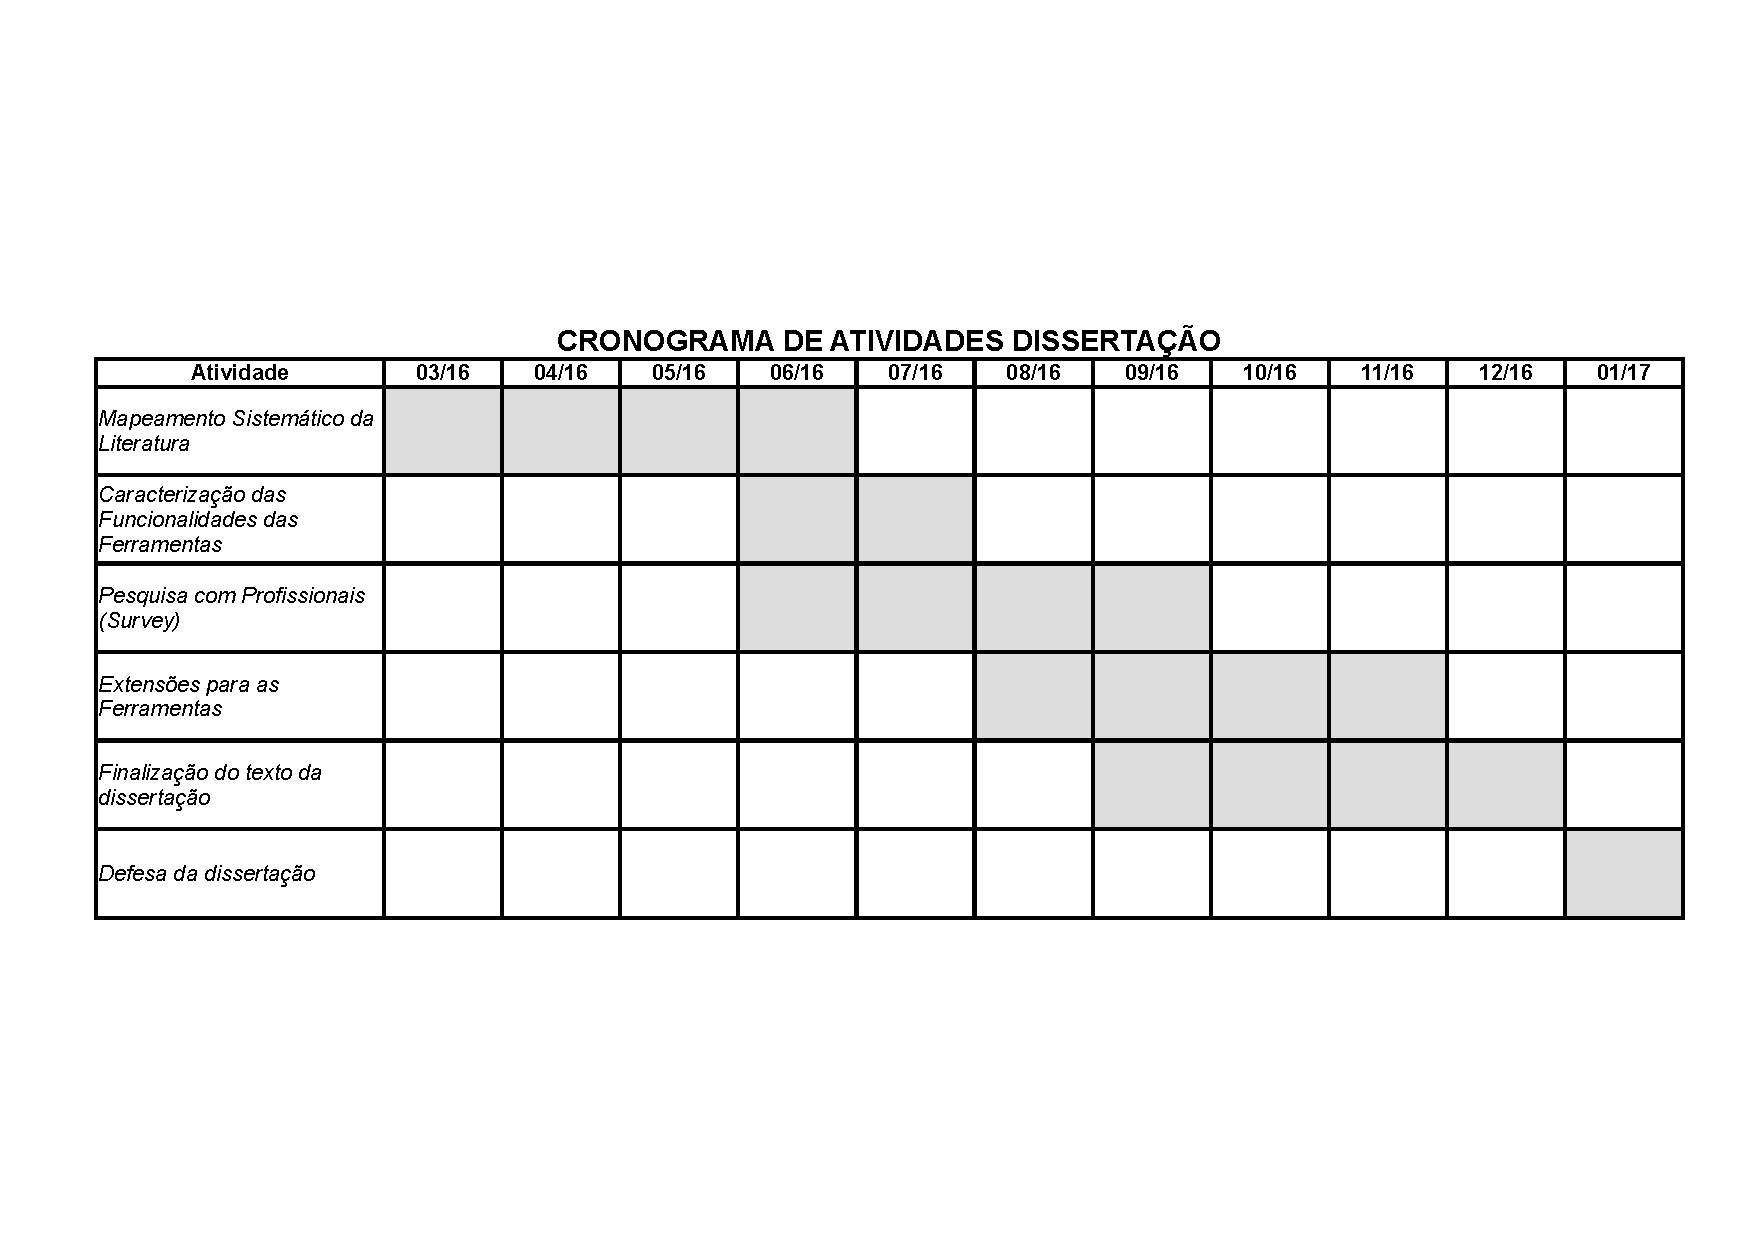
\includepdf{Cronograma-Atividades-Dissertacao.pdf}
 
 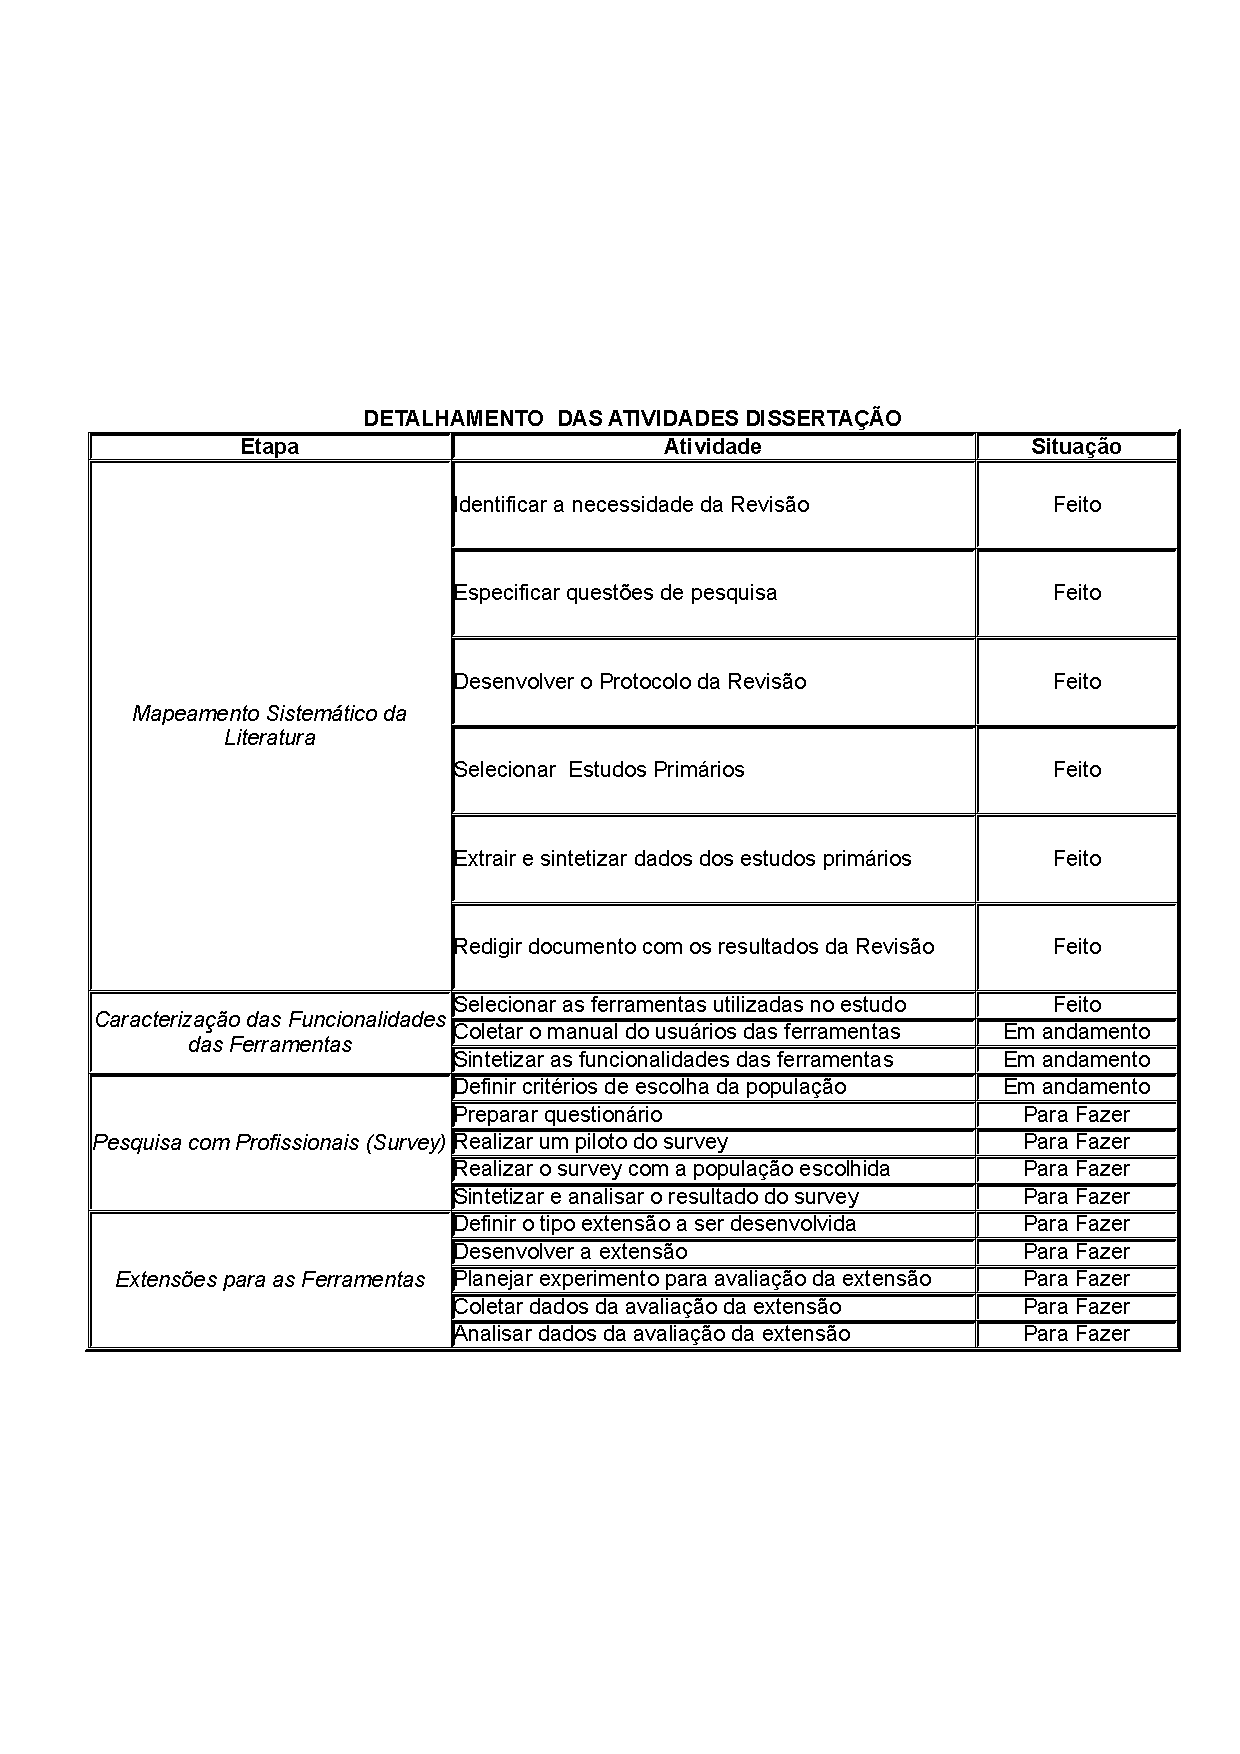
\includepdf{Detalhamento-Atividades-Dissertacao.pdf}

\bibliographystyle{acm}
\bibliography{relatorio}
\end{document}